\chapter{Sampling Between Different Resolutions}
\label{ch:sampling}

%\begin{fquote}[Kurt Lewin] If you truly want to understand something try to change it. \fqsource{German-American Psychologist(1890-1947)} \end{fquote} 
\begin{fquote}[ Ralph Waldo Emerson] For everything you have missed, you have gained something else, and for everything you gain, you lose something else. \fqsource{American Poet, Lecturer and Essayist(1803-1882)} \end{fquote}
\begin{synopsis}
This chapter focuses on the different methods used to upsample data to finer resolutions and downsample data to coarser resolutions. Upsampling, discussed in Section~\ref{s:upsampling}, transforms the resolution of data from coarse to fine. The three downsampling methods discussed in Sections~\ref{ss:weighted},~\ref{ss:orfunction},~and \ref{ss:majority} transform the data from fine resolution to coarse resolution. Part of the work discussed in this chapter has been published in~\cite{premup}.
\end{synopsis}

Sampling resolutions in cytogenetics is a process of defining the level of precision for the staining techniques to produce the results either global or detailed view. A good metaphor for sampling as given by~\cite{scaling} in terms of speech recognition can be an advertisement recently aired in a Dutch Television where the shot is started with a global view. In this case, a shot was taken from the orbit satellite and gradually zooming into Europe, the Netherlands, the Dutch North Sea Coast, the Scheveningen beach up to a lady drinking a glass of beer in a terrace. Similar to the advertisement, different staining techniques produce chromosome bands in different resolution. Computational algorithms can be designed to work with only specific resolution of chromosome band. Hence, upsampling or downsampling is necessary before the data can be fed to the algorithm. Furthermore, comparing the results of an algorithm on data in different resolution can produce interesting results which aid in determining suitable resolution of data. In addition, experiments in different resolutions can be helpful in determining the appropriate method for staining.

\begin{figure}[h!]
\centering
\includegraphics[width=0.9\textwidth]{figures/samplingprocedure}
\caption[Sampling in Multiple Resolution]{Schematic representation of sampling in multiple resolutions where upsampling transforms the data to find resolution while downsampling transforms the data to coarse resolution.} \label{Fig:samplinginmultires}
\end{figure} 

Section~\ref{s:multipleresolutions} explained the problem of multiple resolution in chromosome along with the Figure~\ref{Fig:probmultires} which showed the G-banding pattern of Chromosome~17 in five different resolutions. In the context of Figure~\ref{Fig:probmultires}, upsampling and downsampling can be seen as the process of data transformations as shown by the arrows in Figure~\ref{Fig:samplinginmultires}. Upsampling changes the representation of data from coarse resolution to fine resolution as shown by the arrow pointing to the right in Figure~\ref{Fig:samplinginmultires}. Similarly, downsampling changes the representation of the data from fine resolution to coarse resolution as shown by the arrow pointing to the left in Figure~\ref{Fig:samplinginmultires}.


\section{Upsampling}
\label{s:upsampling}

Upsampling, as shown in Figure~\ref{Fig:upscaling}, is the process of changing the representation of data to the fine resolution. A simple method was devised to upsample the data from coarse resolution. Upsampling was simple and were implemented using simple transformation tables or lookup tables. Initially, the dataset was in resolution 400 and it was upsampled to three different resolutions 550, 700 and 850. Multiple copies of cytogenetic band in coarser resolution were made to upsample the data to finer resolution. For example, cytogenetic band 1q36.1 in resolution 550 has been divided into three bands $1q36.11$, $1q36.12$ and $1q36.13$ in resolution $850$. So, multiple copies of $1q36.1$ was made for all bands $1q36.11$, $1q36.12$ and $1q36.13$ in resolution 850. %Figure \ref{Fig:upscaling} depicts the process of upsampling.

\begin{figure}[h!]
\centering
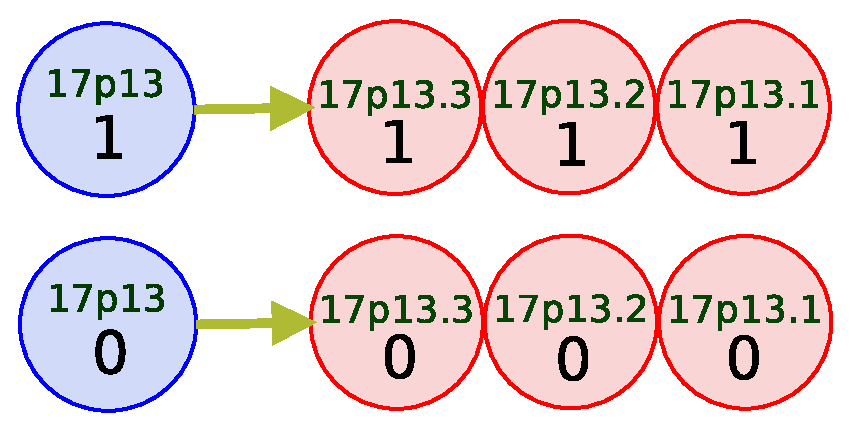
\includegraphics[scale=0.4]{figures/upscaling}
\caption[Upsampling]{Schematic representation of upsampling where duplicate copies of similar cytogenetic bands are made in the finer resolution} \label{Fig:upscaling}
\end{figure}

Figure~\ref{Fig:upscaling} shows that three copies of similar cytogenetic band in coarser resolution are made to upsample the data to finer resolution. When multiple copies of same cytogenetic band is made finer resolution will have only few unique rows. Hence, when the sample size decreases the complex model in higher dimension can not be trained to convergence thus producing poor results. Implementation of downsampling was performed using simple transformation tables implemented in Perl~\cite{perl}. Table~\ref{Tab:Transformation} shows an example of table for transformation of data in 400 resolution to 850 resolution for chromosome 17.

\begin{table}[h!]
  \centering
  \begin{tabular}{|@{}l@{}|@{}l@{}|}
    \hline
    \textbf{Chromosome Resolution 400} & \textbf{Chromosome Resolution 850}  \\
    \hline
    17p13	& 	17p13.3  \\ \hline
    ...		& 	17p13.2  \\ \hline
    ...		& 	17p13.1  \\ \hline
    17p12	& 	17p12 	 \\ \hline
    17p11.2	& 	17p11.2  \\ \hline
    17p11.1	& 	17p11.1  \\ \hline
    17q11.1	& 	17q11.1  \\ \hline
    17q11.2	& 	17q11.2  \\ \hline
    17q12	& 	17q12 	 \\ \hline
    17q21	& 	17q21.1  \\ \hline
    ...		& 	17q21.2  \\ \hline
    ...		& 	17q21.31 \\ \hline
    ...		& 	17q21.32 \\ \hline
    ...		& 	17q21.33 \\ \hline
    17q22	& 	17q22 	 \\ \hline
    17q23	& 	17q23.1  \\ \hline
    ...		& 	17q23.2  \\ \hline
    ...		& 	17q23.3  \\ \hline
    17q24	& 	17q24.1  \\ \hline
    ...		& 	17q24.2  \\ \hline
    ...		& 	17q24.3  \\ \hline
    17q25	& 	17q25.1  \\ \hline
    ...		& 	17q25.2  \\ \hline
    ...		& 	17q25.3  \\ \hline   
  \end{tabular}
  \caption[Example transformation table in chromosome 17 ]{Chromosome bands for resolution 400 \& 850 and their transformation} \label{Tab:Transformation}
\end{table}

Table~\ref{Tab:Transformation} shows that some chromosome bands missing in 400 resolution are observed in resolution 850. Hence, duplicate copies of the similar chromosome band in resolution 400 were made in finer resolution. Duplications are made based on the assumption that if an adjacent area is amplified then the probability of the chromosome band being amplified is high because amplifications typically cover large areas. The transformation table were chromosome specific and resolution specific (i.e. 88 transformation tables in all for different chromosomes). 

\section{Downsampling}
\label{s:downsampling}
Downsampling is the process of changing the representation of the data to the coarser resolution. In both cases of upsampling and downsampling, no attempt is made to infer the structure of the data and no information is added or removed during the process. If the data of the same patients were available in two different resolutions, one of the supervised classification algorithms in machine learning could be used in downsampling dealing the problem as a traditional classification problem. However, such data was not available. Hence, simple but useful methods motivated from biology are used for downsampling. Downsampling methods were implemented in scripts with a script for each chromosome in each resolution. Sections~\ref{ss:orfunction},~\ref{ss:majority} and~\ref{ss:weighted} detail the methods of downsampling. %Interestingly, in some cases there were some cytogenetic bands which were not available in finer resolution. For instance, the $q$ arm of chromosome-4 in resolution 850 is divided into $4q35.1$ and $4q35.2$. In contrast, in resolution 700, the $q$ arm of chromosome -4 is divided into three bands: $4q35.1$, $4q35.2$ and $4q35.3$. respectively. In such cases, missing band in coarser resolution was assigned the amplification pattern of its nearest neighbor in all three methods. For the example case above, the cytogenetic band $4q35.3$ was assigned the amplification pattern of $4q35.2$.

\subsection{OR-function Downsampling}
\label{ss:orfunction}

\begin{figure}[h!]
\centering
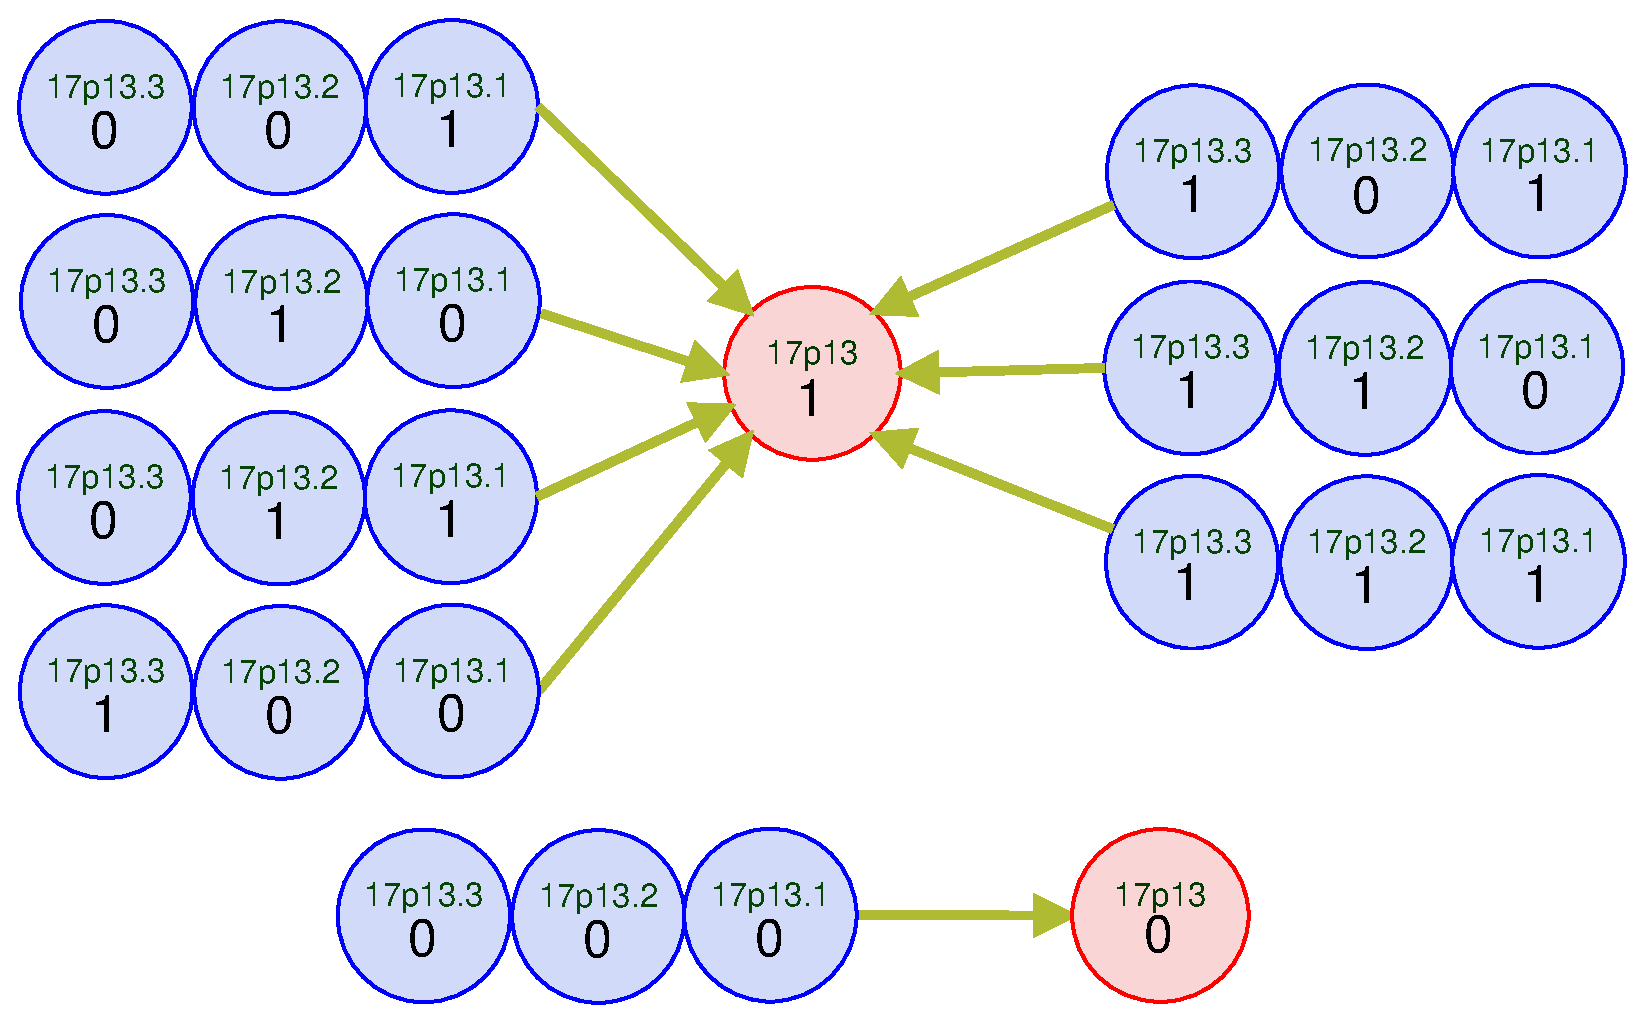
\includegraphics[scale=0.35]{figures/ptmapping}
\caption[OR-function downsampling]{{Schematic representation of OR-function downsampling procedure. Here the cytogenetic band in coarser resolution is amplified if any of the bands in finer resolution is amplified. Cytogenetic band in coarser resolution is not amplified only when none of the bands in finer resolution is amplified.}}\label{Fig:ptmapping}
\end{figure}

In  OR-function downsampling method, the cytogenetic band in coarser resolution is not amplified if none of the bands in finer resolution are amplified. The cytogenetic band in coarser resolution is amplified if either of the bands in finer resolution is amplified. Figure~\ref{Fig:ptmapping} depicts the OR-function downsampling method. The OR-function downsampling method is based on simple belief that if the one of the bands in finer resolution is amplified, it signifies the presence of amplification in the band. For the case in the Figure~\ref{Fig:ptmapping} downsampling can be considered as a simple 0-1 classification problem in machine learning where input is three dimensional 0-1 variable and output is one dimensional 0-1 variable. The solution is a simple truth table describing the classical OR operation. This method does not consider the length of the cytogenetic bands.

\subsection{Majority Decision Downsampling}
\label{ss:majority}

\begin{figure}[h!]
\centering
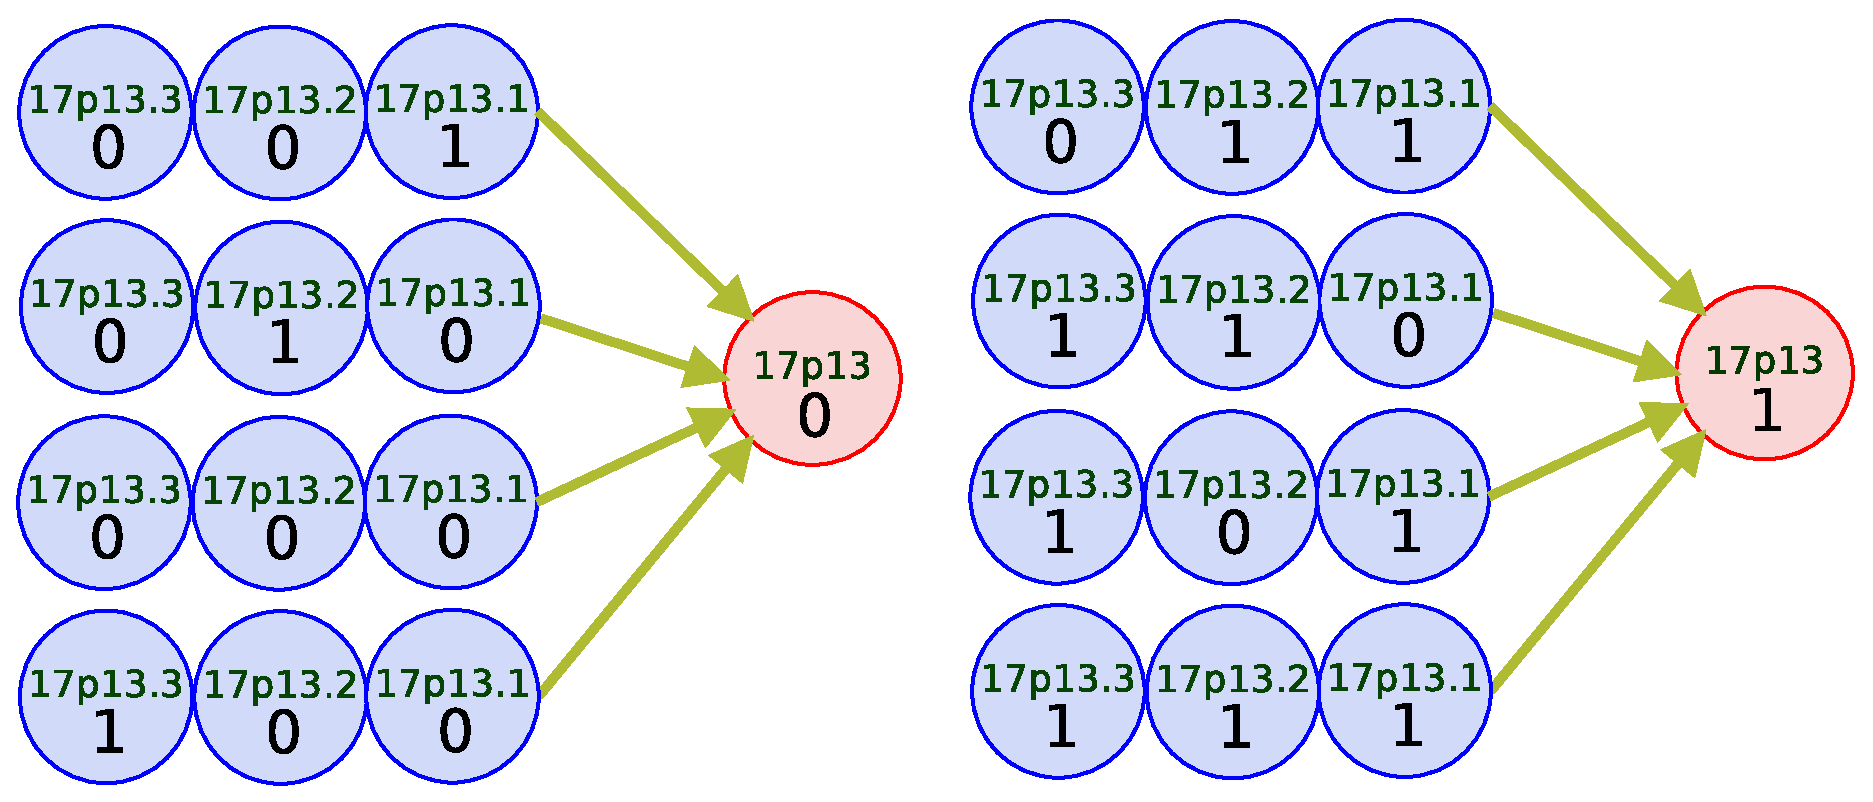
\includegraphics[scale=0.35]{figures/mdmapping.eps}
\caption[Majority decision downsampling]{Schematic representation of majority decision downsampling procedure. Here the cytogenetic band in coarser resolution is amplified if majority of the bands in finer resolution are amplified, otherwise it not amplified.} \label{Fig:mdmapping}
\end{figure}

In majority decision downsampling method, a cytogenetic band in coarser resolution is amplified if majority of the cytogenetic bands in finer resolution are amplified otherwise the cytogenetic band is not amplified. In case of a tie amplification of two nearest bands one in the left and the other one in the right are taken into consideration iteratively and the amplification pattern of the band is determined using the idea similar to `golden goal'\footnote{The golden goal is a method used in football to determine the winner which end in a draw after the end of regulation time. Golden goal rules allow the team that scores the first goal during extra time to be declared the winner. The game finishes when a golden goal is scored.} strategy used in football. In other words, if in any iteration both bands in neighborhood bands are amplified then the band is amplified and if both the neighbors are unamplified then the band is deemed unamplified. If the amplification of coarser resolution can not be concluded with `golden goal' strategy then the band in coarser resolution is deemed as amplified. Figure~\ref{Fig:mdmapping} shows one of the examples of majority decision in downsampling. There is a shortcoming in this downsampling method because it does not take into consideration the the lengths of the cytogenetic bands. The lengths of cytogentenic bands are considered by length weighted downsampling method discussed in Section~\ref{ss:weighted}.

\subsection{Length Weighted Downsampling}
\label{ss:weighted}

\begin{figure}[h!]
\centering
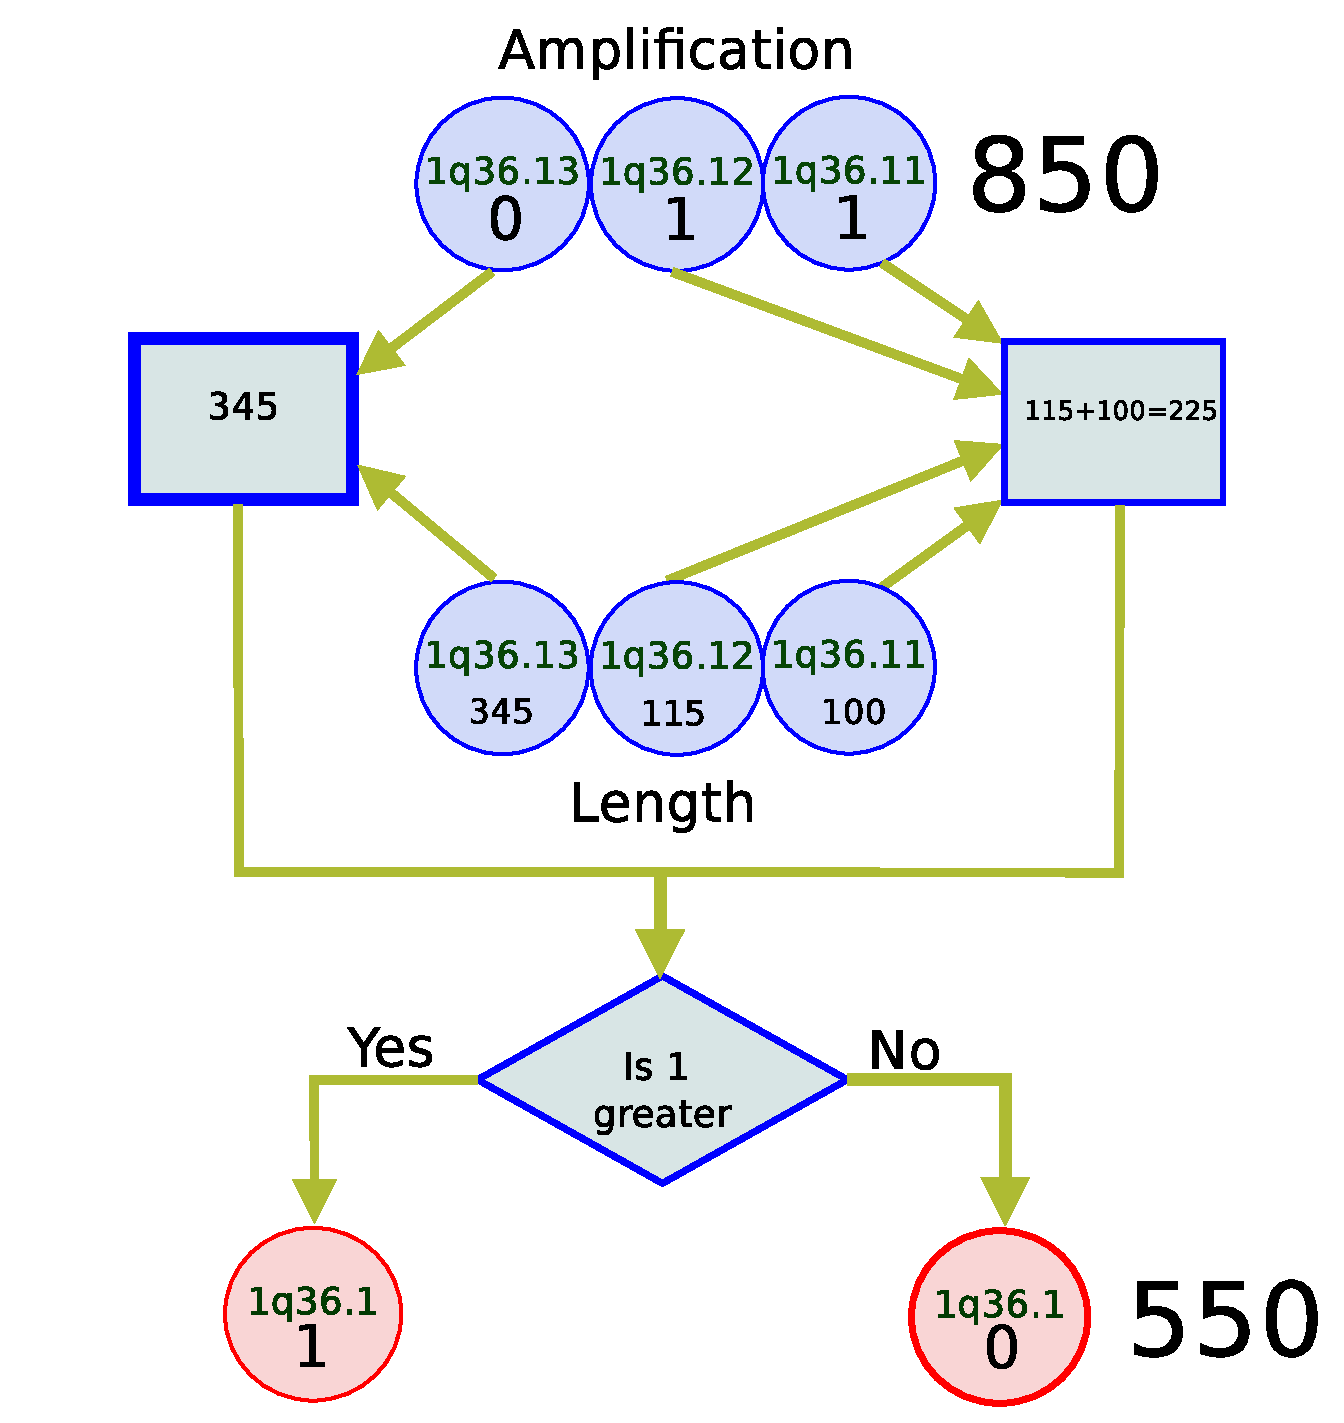
\includegraphics[scale=0.35]{figures/weighted}
\caption[Weighted downsampling]{Schematic representation of weighted downsampling procedure. Here the cytogenetic band in coarser resolution is amplified if total length of the  amplified bands in finer resolution is greater than the total length of unamplified bands, otherwise it not amplified. The figure is an example case in chromosome 1q36.1 where two cytogenetic bands 1q36.11 and 1q36.12 in resolution 850 are amplified and one band 1q36.13 is not amplified. However, total length of unamplified region i.e. band 1q36.13 (345) is greater than total length of the unamplified region i.e. bands 1q36.11 and 1q36.12 (100+115=225). Hence, the band in resolution 550 is unamplified.} \label{Fig:wamapping}
\end{figure} 

In length weighted downsampling method, depicted in the Figure~\ref{Fig:wamapping}, length of the cytogenetic band is considered. The length of the cytogenetic band varies in each assembly and hence relative lengths were considered. The amplification of cytogenetic band in coarser resolution is determined by the weighted length of cytogenetic band in finer resolution. Each cytogenetic band is weighted according to the relative length of the cytogenetic band. If the total length of amplified region is greater than the total length of unamplified region, the cytogenetic band in coarser resolution is amplified, otherwise the cytogenetic band is unamplified. Here, relative length is considered which gives more accurate measure of the amplification profiles in the cytogenetic band. Absolute lengths of the cytogenetic bands are currently not available and vary with each assembly. Two relative measures were considered in the calculation of the length. From the ideogram dataset available in NCBI~\cite{ncbi}, the difference between ISCN.top and ISCN.bot were used as relative measures. Similarly, difference between bases-top and bases-bot were also used as the relative measure of the length of each cytogenetic band. The difference in the results produced using the different relative measure of length have also been studied. 





